
\section*{RUP: Rational Unified Process}

La metodolog�a utilizada para la elaboraci�n de este proyecto ha sido 
\emph{RUP}\footnote{\url{http://www.rational.com/products/rup/}}
(Rational Unified Process, Proceso Racional Unificado) de IBM.

La raz�n principal fue la genericidad que brinda para el proceso de desarrollo
software, adaptandose perfectamente a desarrollos basados en programaci�n 
orientada a objetos.

Ayudo a implementar determinadas buenas pr�cticas en Ingenier�a del Software:

\begin{itemize}
  \item Desarrollo iterativo
  \item Administraci�n de requisitos
  \item Uso de arquitectura basada en componentes
  \item Control de cambios
  \item Verificaci�n de la calidad del software
\end{itemize}

Por tanto todo el proceso de desarrollo se dividi� en ciclos, teniendo un 
producto final al final de cada ciclo, dividiendo cada ciclo en fases que 
finalizan con un hito importante.

\begin{figure}[ht]
	\centering
	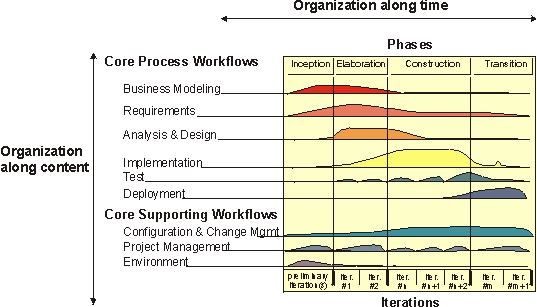
\includegraphics[width=12cm]{images/rup.png}
	\caption{Vista general de RUP}
	\label{fig:RUP}
\end{figure}

Los fases seguidas fueron:

\begin{enumerate}
  \item Inicio: se hizo un plan de fases, identificando los principales 
	casos de uso y riesgos.
  \item Elaboraci�n: se hizo un plan de proyecto, completandose los casos 
	de uso para eliminar los riesgos.
  \item Construcci�n: se concentro en la elaboraci�n de un producto totalmente 
	operativo y eficiente, asicomo en un peque�o manual de usuario.
  \item Transici�n: se implemento el producto en el cliente y se publicaron
	varias versiones funcionales. Como consecuencia de esta publicaci�n
	surgieron nuevos requisitos a ser analizados.
\end{enumerate}

Para cada fase RUP define nueve actividades a realizar:

\begin{enumerate}
 \item Modelado del negocio
 \item An�lisis de requisitos
 \item An�lisis y dise�o
 \item Implementaci�n
 \item Test
 \item Distribuci�n
 \item Gesti�n de configuraci�n y cambios
 \item Gesti�n del proyecto
 \item Gesti�n del entorno
\end{enumerate}

Adem�s de un flujo de trabajo entre ellas:

\begin{figure}[ht]
	\centering
	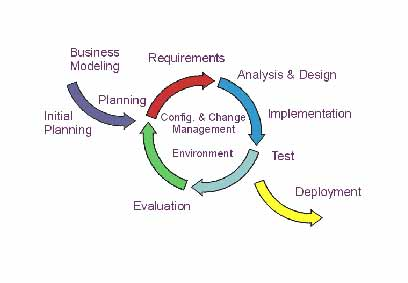
\includegraphics[width=9cm]{images/workflow-rup.png}
	\caption{Flujos de trabajo de RUP}
	\label{fig:RUP}
\end{figure}

En RUP de utiliza UML\footnote{\url{http://www.omg.org/uml/}} como herramienta principal
para la documentaci�n de toda la arquitectura del sistema. La bibliografia es amplia,
disponiendo de veteranos t�tulos como 
\emph{The Unified Modeling Language Reference Manual}\cite{UMLReference} o 
\emph{UML Distilled}\cite{UMLDistilled} como guias de referencia, siendo imprescidible
tener siempre a mano el \emph{UML 2.0 Pocket Reference}\cite{UMLPocket} para resolver
r�pidamente esas consultas puntuales de la especificaci�n.

RUP puede englobarse dentro de lo que algunos llaman \emph{procesos pesados},
estando quiz�s muy orientado para proyecto de algo m�s de envergadura que SWAML.
Es por ello que debido a las caracteristicas del proyecto, tama�o y personas 
involucradas, se ha adaptado RUP utilizando s�lo los documentos y procesos de 
dise�os necesarios.

Este m�todo es de sobra conocido y esta perfectamente documentado (en libros como
\emph{The Rational Unified Process}\cite{RUPIntro} y
\emph{The Rational Unified Process Made Easy}\cite{RUPEasy}) como para
extenderse m�s reescribiendo dicha documentaci�n.
